\input{Configuraciones/paquetes}

%--------------------------

\begin{document}
\input{Configuraciones/nombres}
%--------------------------


\begin{problema}
    Sea $f$ analítica en el interior y sobre el rectángulo $R$ dado: 
    \begin{figure}[H]
        \centering


\tikzset{every picture/.style={line width=0.75pt}} %set default line width to 0.75pt        

\begin{tikzpicture}[x=0.75pt,y=0.75pt,yscale=-1,xscale=1]
%uncomment if require: \path (0,300); %set diagram left start at 0, and has height of 300

%Shape: Rectangle [id:dp45604917113398014] 
\draw   (190.2,88) -- (438.2,88) -- (438.2,201.4) -- (190.2,201.4) -- cycle ;

% Text Node
\draw (176,73) node [anchor=north west][inner sep=0.75pt]   [align=left] {A};
% Text Node
\draw (177,202) node [anchor=north west][inner sep=0.75pt]   [align=left] {B};
% Text Node
\draw (440.2,204.4) node [anchor=north west][inner sep=0.75pt]   [align=left] {C};
% Text Node
\draw (439.2,73.4) node [anchor=north west][inner sep=0.75pt]   [align=left] {D};


\end{tikzpicture}
    \end{figure}
    Entonces $\int_R f=0$.
\end{problema}

\begin{dem}
    Sea, $P$ el perímetro de $R$ y $d$ la longitud de su diagonal. Sea entonces 
    \begin{figure}[H]
        \centering 
        

\tikzset{every picture/.style={line width=0.75pt}} %set default line width to 0.75pt        

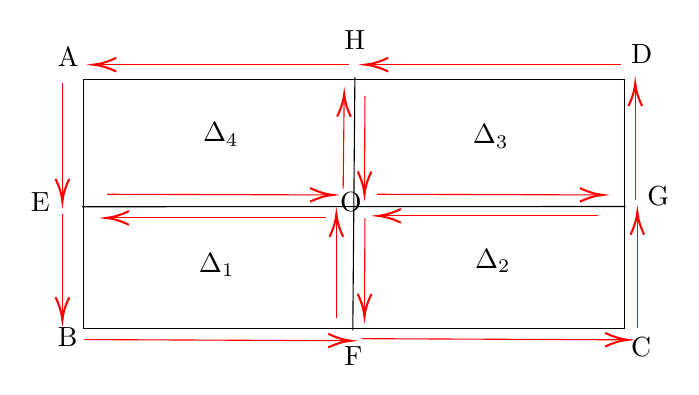
\begin{tikzpicture}[x=0.75pt,y=0.75pt,yscale=-1,xscale=1]
%uncomment if require: \path (0,300); %set diagram left start at 0, and has height of 300

%Shape: Rectangle [id:dp45604917113398014] 
\draw   (189.59,89.57) -- (450.17,89.57) -- (450.17,209.57) -- (189.59,209.57) -- cycle ;
%Straight Lines [id:da4438737457776333] 
\draw    (189,151) -- (450.79,150.9) ;
%Straight Lines [id:da7524672749913988] 
\draw    (319.38,210.57) -- (320.38,88.57) ;
%Straight Lines [id:da02361708569917431] 
\draw [color={rgb, 255:red, 255; green, 0; blue, 0 }  ,draw opacity=1 ]   (201,145) -- (307.73,145.31) ;
\draw [shift={(309.73,145.32)}, rotate = 180.17] [color={rgb, 255:red, 255; green, 0; blue, 0 }  ,draw opacity=1 ][line width=0.75]    (10.93,-3.29) .. controls (6.95,-1.4) and (3.31,-0.3) .. (0,0) .. controls (3.31,0.3) and (6.95,1.4) .. (10.93,3.29)   ;
%Straight Lines [id:da6113383562830937] 
\draw [color={rgb, 255:red, 255; green, 0; blue, 0 }  ,draw opacity=1 ]   (314.73,142.32) -- (315.21,98.65) ;
\draw [shift={(315.23,96.65)}, rotate = 90.63] [color={rgb, 255:red, 255; green, 0; blue, 0 }  ,draw opacity=1 ][line width=0.75]    (10.93,-3.29) .. controls (6.95,-1.4) and (3.31,-0.3) .. (0,0) .. controls (3.31,0.3) and (6.95,1.4) .. (10.93,3.29)   ;
%Straight Lines [id:da8536399840374138] 
\draw [color={rgb, 255:red, 255; green, 0; blue, 0 }  ,draw opacity=1 ]   (331,145) -- (437.73,145.31) ;
\draw [shift={(439.73,145.32)}, rotate = 180.17] [color={rgb, 255:red, 255; green, 0; blue, 0 }  ,draw opacity=1 ][line width=0.75]    (10.93,-3.29) .. controls (6.95,-1.4) and (3.31,-0.3) .. (0,0) .. controls (3.31,0.3) and (6.95,1.4) .. (10.93,3.29)   ;
%Straight Lines [id:da5720939819490577] 
\draw [color={rgb, 255:red, 255; green, 0; blue, 0 }  ,draw opacity=1 ]   (325.23,97.65) -- (325.01,143) ;
\draw [shift={(325,145)}, rotate = 270.28] [color={rgb, 255:red, 255; green, 0; blue, 0 }  ,draw opacity=1 ][line width=0.75]    (10.93,-3.29) .. controls (6.95,-1.4) and (3.31,-0.3) .. (0,0) .. controls (3.31,0.3) and (6.95,1.4) .. (10.93,3.29)   ;
%Straight Lines [id:da005641798815771426] 
\draw [color={rgb, 255:red, 255; green, 0; blue, 0 }  ,draw opacity=1 ]   (190,215) -- (316.46,215.56) ;
\draw [shift={(318.46,215.56)}, rotate = 180.25] [color={rgb, 255:red, 255; green, 0; blue, 0 }  ,draw opacity=1 ][line width=0.75]    (10.93,-3.29) .. controls (6.95,-1.4) and (3.31,-0.3) .. (0,0) .. controls (3.31,0.3) and (6.95,1.4) .. (10.93,3.29)   ;
%Straight Lines [id:da3141379957715388] 
\draw [color={rgb, 255:red, 255; green, 0; blue, 0 }  ,draw opacity=1 ]   (306.6,156.4) -- (202.6,156.4) ;
\draw [shift={(200.6,156.4)}, rotate = 360] [color={rgb, 255:red, 255; green, 0; blue, 0 }  ,draw opacity=1 ][line width=0.75]    (10.93,-3.29) .. controls (6.95,-1.4) and (3.31,-0.3) .. (0,0) .. controls (3.31,0.3) and (6.95,1.4) .. (10.93,3.29)   ;
%Straight Lines [id:da9351399140326178] 
\draw [color={rgb, 255:red, 255; green, 0; blue, 0 }  ,draw opacity=1 ]   (311.46,204.56) -- (311.46,156.56) ;
\draw [shift={(311.46,154.56)}, rotate = 90] [color={rgb, 255:red, 255; green, 0; blue, 0 }  ,draw opacity=1 ][line width=0.75]    (10.93,-3.29) .. controls (6.95,-1.4) and (3.31,-0.3) .. (0,0) .. controls (3.31,0.3) and (6.95,1.4) .. (10.93,3.29)   ;
%Straight Lines [id:da1365389682217346] 
\draw [color={rgb, 255:red, 255; green, 0; blue, 0 }  ,draw opacity=1 ]   (437.6,155.4) -- (333.6,155.4) ;
\draw [shift={(331.6,155.4)}, rotate = 360] [color={rgb, 255:red, 255; green, 0; blue, 0 }  ,draw opacity=1 ][line width=0.75]    (10.93,-3.29) .. controls (6.95,-1.4) and (3.31,-0.3) .. (0,0) .. controls (3.31,0.3) and (6.95,1.4) .. (10.93,3.29)   ;
%Straight Lines [id:da3232602977758703] 
\draw [color={rgb, 255:red, 255; green, 0; blue, 0 }  ,draw opacity=1 ]   (325.23,156.65) -- (325.01,202) ;
\draw [shift={(325,204)}, rotate = 270.28] [color={rgb, 255:red, 255; green, 0; blue, 0 }  ,draw opacity=1 ][line width=0.75]    (10.93,-3.29) .. controls (6.95,-1.4) and (3.31,-0.3) .. (0,0) .. controls (3.31,0.3) and (6.95,1.4) .. (10.93,3.29)   ;
%Straight Lines [id:da9474905795484069] 
\draw [color={rgb, 255:red, 255; green, 0; blue, 0 }  ,draw opacity=1 ]   (323.46,214.56) -- (449.92,215.12) ;
\draw [shift={(451.92,215.13)}, rotate = 180.25] [color={rgb, 255:red, 255; green, 0; blue, 0 }  ,draw opacity=1 ][line width=0.75]    (10.93,-3.29) .. controls (6.95,-1.4) and (3.31,-0.3) .. (0,0) .. controls (3.31,0.3) and (6.95,1.4) .. (10.93,3.29)   ;
%Straight Lines [id:da535242801767332] 
\draw [color={rgb, 255:red, 255; green, 0; blue, 0 }  ,draw opacity=1 ]   (456.46,209.56) -- (456.46,155.56) ;
\draw [shift={(456.46,153.56)}, rotate = 90] [color={rgb, 255:red, 255; green, 0; blue, 0 }  ,draw opacity=1 ][line width=0.75]    (10.93,-3.29) .. controls (6.95,-1.4) and (3.31,-0.3) .. (0,0) .. controls (3.31,0.3) and (6.95,1.4) .. (10.93,3.29)   ;
%Straight Lines [id:da741266639730476] 
\draw [color={rgb, 255:red, 255; green, 0; blue, 0 }  ,draw opacity=1 ]   (455.46,147.56) -- (455.46,93.56) ;
\draw [shift={(455.46,91.56)}, rotate = 90] [color={rgb, 255:red, 255; green, 0; blue, 0 }  ,draw opacity=1 ][line width=0.75]    (10.93,-3.29) .. controls (6.95,-1.4) and (3.31,-0.3) .. (0,0) .. controls (3.31,0.3) and (6.95,1.4) .. (10.93,3.29)   ;
%Straight Lines [id:da10946242409855389] 
\draw [color={rgb, 255:red, 255; green, 0; blue, 0 }  ,draw opacity=1 ]   (448.46,82.56) -- (327.46,82.56) ;
\draw [shift={(325.46,82.56)}, rotate = 360] [color={rgb, 255:red, 255; green, 0; blue, 0 }  ,draw opacity=1 ][line width=0.75]    (10.93,-3.29) .. controls (6.95,-1.4) and (3.31,-0.3) .. (0,0) .. controls (3.31,0.3) and (6.95,1.4) .. (10.93,3.29)   ;
%Straight Lines [id:da6947988816572367] 
\draw [color={rgb, 255:red, 255; green, 0; blue, 0 }  ,draw opacity=1 ]   (317.46,82.56) -- (196.46,82.56) ;
\draw [shift={(194.46,82.56)}, rotate = 360] [color={rgb, 255:red, 255; green, 0; blue, 0 }  ,draw opacity=1 ][line width=0.75]    (10.93,-3.29) .. controls (6.95,-1.4) and (3.31,-0.3) .. (0,0) .. controls (3.31,0.3) and (6.95,1.4) .. (10.93,3.29)   ;
%Straight Lines [id:da7639576063262005] 
\draw [color={rgb, 255:red, 255; green, 0; blue, 0 }  ,draw opacity=1 ]   (179.46,91.56) -- (179.46,146.56) ;
\draw [shift={(179.46,148.56)}, rotate = 270] [color={rgb, 255:red, 255; green, 0; blue, 0 }  ,draw opacity=1 ][line width=0.75]    (10.93,-3.29) .. controls (6.95,-1.4) and (3.31,-0.3) .. (0,0) .. controls (3.31,0.3) and (6.95,1.4) .. (10.93,3.29)   ;
%Straight Lines [id:da21910362747323675] 
\draw [color={rgb, 255:red, 255; green, 0; blue, 0 }  ,draw opacity=1 ]   (179.46,154.56) -- (179.46,203.56) ;
\draw [shift={(179.46,205.56)}, rotate = 270] [color={rgb, 255:red, 255; green, 0; blue, 0 }  ,draw opacity=1 ][line width=0.75]    (10.93,-3.29) .. controls (6.95,-1.4) and (3.31,-0.3) .. (0,0) .. controls (3.31,0.3) and (6.95,1.4) .. (10.93,3.29)   ;

% Text Node
\draw (176,73) node [anchor=north west][inner sep=0.75pt]   [align=left] {A};
% Text Node
\draw (176,208) node [anchor=north west][inner sep=0.75pt]   [align=left] {B};
% Text Node
\draw (452.17,212.57) node [anchor=north west][inner sep=0.75pt]   [align=left] {C};
% Text Node
\draw (452.2,71.4) node [anchor=north west][inner sep=0.75pt]   [align=left] {D};
% Text Node
\draw (244,172.4) node [anchor=north west][inner sep=0.75pt]    {$\Delta _{1}$};
% Text Node
\draw (377,170.4) node [anchor=north west][inner sep=0.75pt]    {$\Delta _{2}$};
% Text Node
\draw (376,110.4) node [anchor=north west][inner sep=0.75pt]    {$\Delta _{3}$};
% Text Node
\draw (246,109.4) node [anchor=north west][inner sep=0.75pt]    {$\Delta _{4}$};
% Text Node
\draw (163,143) node [anchor=north west][inner sep=0.75pt]   [align=left] {E};
% Text Node
\draw (314,217) node [anchor=north west][inner sep=0.75pt]   [align=left] {F};
% Text Node
\draw (460,140) node [anchor=north west][inner sep=0.75pt]   [align=left] {G};
% Text Node
\draw (314,65) node [anchor=north west][inner sep=0.75pt]   [align=left] {H};
% Text Node
\draw (312,143) node [anchor=north west][inner sep=0.75pt]   [align=left] {O};


\end{tikzpicture}
    \end{figure}
    De esto, tenemos: 
    \begin{align*}
        \int_{R}f =\int_{ABCD}f &= \int_{HAE}f+\int_{EBF}f+\int_{FCG}f+\int_{GDH}f\\
        &= \left[\int_{HAE}f+\int_{EO}f+\int_{OH}f\right] + \left[\int_{EBF}f+\int_{FO}f-\int_{EO}f\right]\\
        &+\left[\int_{FCG}f+\int_{GO}f-\int_{FO}f\right]+\left[\int_{GDH}f-\int_{OH}f-\int_{GO}f\right]\\
        &= \left[\int_{HAE}f+\int_{EO}f+\int_{OH}f\right] + \left[\int_{EBF}f+\int_{FO}f+\int_{OE}f\right]\\
        &+\left[\int_{FCG}f+\int_{GO}f+\int_{OF}f\right]+\left[\int_{GDH}f+\int_{HO}f+\int_{OG}f\right]\\
        &= \oint_{HAEOH}f+\oint_{EBFOE}f+\oint_{FCGOF}f+\oint_{GDHOG}f\\
        &= \oint_{\Delta_4}f + \oint_{\Delta_1}f+\oint_{\Delta_2}f+\oint_{\Delta_3}f
    \end{align*}
    De esto, 
    \begin{align*}
        \left|\oint_{R} f(z)dz\right|\leq \left|\oint_{\Delta_1} f(z)dz\right|+\left|\oint_{\Delta_2} f(z)dz\right|+\left|\oint_{\Delta_3} f(z)dz\right|+\left|\oint_{\Delta_4} f(z)dz\right|
    \end{align*}
    
    Ahora bien, definimos:
    $$\left|\oint_{R_1}f(x)dx\right|=\max_{i\in \{1,2,3,4\}}\left|\oint_{\Delta_i}f(z)dz\right|$$

        $$\frac{1}{4}\left|\oint_{R}f(z)dz\right| \leq \left|\oint_{R_1}f(z)dz\right|$$
        \begin{cajita}
            El perímetro y diagonal de $R_1$ son la mitad de $R$. 
        \end{cajita}

        \begin{figure}[H]
            \centering
            

\tikzset{every picture/.style={line width=0.75pt}} %set default line width to 0.75pt        

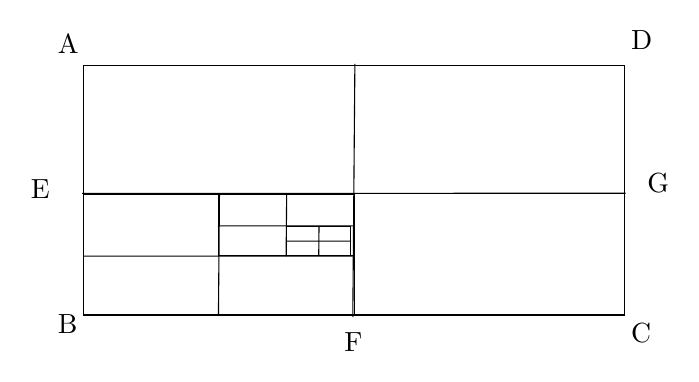
\begin{tikzpicture}[x=0.75pt,y=0.75pt,yscale=-1,xscale=1]
%uncomment if require: \path (0,300); %set diagram left start at 0, and has height of 300

%Shape: Rectangle [id:dp45604917113398014] 
\draw   (189.59,89.57) -- (450.17,89.57) -- (450.17,209.57) -- (189.59,209.57) -- cycle ;
%Straight Lines [id:da4438737457776333] 
\draw    (189,151) -- (450.79,150.9) ;
%Straight Lines [id:da7524672749913988] 
\draw    (319.38,210.57) -- (320.38,88.57) ;
%Shape: Rectangle [id:dp31703544369839554] 
\draw   (189.69,151.48) -- (320.09,151.48) -- (320.09,209.52) -- (189.69,209.52) -- cycle ;
%Straight Lines [id:da3505939428066783] 
\draw    (189.4,181.19) -- (320.4,181.15) ;
%Straight Lines [id:da847948366563795] 
\draw    (254.64,210) -- (255.14,151) ;
%Shape: Rectangle [id:dp8520514946196467] 
\draw   (254.54,151.52) -- (320.24,151.52) -- (320.24,181.03) -- (254.54,181.03) -- cycle ;
%Straight Lines [id:da7408182191618652] 
\draw    (254.39,166.62) -- (320.39,166.6) ;
%Straight Lines [id:da1354943908628089] 
\draw    (287.26,181.27) -- (287.51,151.27) ;
%Shape: Rectangle [id:dp5520186097047262] 
\draw   (287.6,166.95) -- (318.45,166.95) -- (318.45,180.72) -- (287.6,180.72) -- cycle ;
%Straight Lines [id:da20588935542535214] 
\draw    (287.53,174) -- (318.53,173.98) ;
%Straight Lines [id:da8135218935256636] 
\draw    (302.97,180.83) -- (303.09,166.83) ;

% Text Node
\draw (176,73) node [anchor=north west][inner sep=0.75pt]   [align=left] {A};
% Text Node
\draw (176,208) node [anchor=north west][inner sep=0.75pt]   [align=left] {B};
% Text Node
\draw (452.17,212.57) node [anchor=north west][inner sep=0.75pt]   [align=left] {C};
% Text Node
\draw (452.2,71.4) node [anchor=north west][inner sep=0.75pt]   [align=left] {D};
% Text Node
\draw (163,143) node [anchor=north west][inner sep=0.75pt]   [align=left] {E};
% Text Node
\draw (314,217) node [anchor=north west][inner sep=0.75pt]   [align=left] {F};
% Text Node
\draw (460,140) node [anchor=north west][inner sep=0.75pt]   [align=left] {G};


\end{tikzpicture}          
        \end{figure}

        Repitiendo este proceso para $R_i$, se tiene que:
        $$\frac{1}{4}\left|\oint_{R_1}f(x)dx\right| \leq \left|\oint_{R_2}f(z)dz\right|$$
        $$\implies \frac{1}{4^2}\left|\oint_{R}f(x)dx\right| \leq \left|\oint_{R_2}f(z)dz\right|$$
        Luego de $n$ etapas en este procesos: 
        $$\frac{1}{4^n}\left|\oint_{R}f(x)dx\right| \leq \left|\oint_{R_n}f(z)dz\right|$$

        Este proceso de bisección lo podemos resumir en 3 aspectos: 
        \begin{enumerate}
            \item $\left|\oint_{R_n}f\right|\geq \frac{1}{4}\left|\oint_{R_n -1}f\right| \geq \cdots \geq \frac{1}{4^n}\left|\oint_R f\right|$
            \item Perímetros:
                \begin{enumerate}
                    \item Perímetro($R_n$)$=\frac{1}{2^n}$
                    \item Perímetro($R$)$=\frac{P}{2^n}$.
                \end{enumerate}
            \item Diagonales: 
            \begin{enumerate}
                \item Diagonal($R_n$)$=\frac{1}{2^n}$
                \item Diagonal($R$)$=\frac{d}{2^n}$
            \end{enumerate}
        \end{enumerate}

        \begin{cajita}
            Nótese que $R\supset R_1\supset R_2\supset R \cdots\supset R_n,\cdots $. Es decir, se tiene una sucesión anidada de rectángulos. Esto quiere decir que existe un punto $z_0$ que pertenece a todos los rectángulos. 
        \end{cajita}

        \begin{cajita}
            \begin{lema}
                Sea $f$ analítica en una región $R$ que contiene al punto $z_0$. Entonces, 
                $$f(z)=f(z_0)+f'(z_0)(z-z_0)+\eta (z-z_0),$$
                donde $\eta\to 0$ cuando $z\to z_0$.
                \begin{dem}
                    Sea $\eta=\frac{f(z)-f(z_0)}{z-z_0}-f'(z_0)$. Como $f$ es diferenciable en $z_0$, entonces si $z\to z_0\implies \eta=0$. Por lo tanto, $f(z)=f(z_0)+f'(z_0)(z-z_0)+\eta(z-z_0)$
                \end{dem}
            \end{lema}
        \end{cajita}
        Como $f$ es analítica en $z_0$, entonces: 
        $$f(z)=f(z_0)+f'(z_0)*(z-z_0)+\eta(z-z_0),$$
        donde, se cumple que, $\forall \varepsilon >0\exists \delta>0\ni |\eta|<\varepsilon$, cuando $|z-z_0|<\frac{d}{2^n}<\delta$. 
        

        Ahora bien, 

        \begin{align*}
            \left|\oint_{R_n}f(z)dz\right|&\leq 4^n\left|\int_{R_n}f\right|\\
            &= 4^n\left|\oint_{R_n}f(z_0)dz+f'(z_0)\oint_{R_n}(z-z_0)dz+\oint_{\Delta_n}\eta(z-z_0)dz\right|\\
            &= 4^n\left|\oint_{R_n}\eta(z-z_0)\right|dz\\
            &\leq 4^n\left|\eta\right|\left|(z-z_0)\right|\cdot l(R_n)\\
            &< 4^n\left(\varepsilon\frac{d}{2^n}\right)\cdot \text{Perímetro}(R_n)\\
            &= 4^n\left(\varepsilon\frac{d}{2^n}\right)\cdot \frac{1}{2^n}\\
            &< 4^n\left(\varepsilon\frac{d}{2^n}\right)\cdot \frac{P}{2^n}\\
            &= \varepsilon dP 
        \end{align*}
        Como $\varepsilon$ era arbitrario, entonces $\left|\int_R f\right|=0$ y por lo tanto, $\int_R f =0$.
    
\end{dem}

%---------------------------
%\bibliographystyle{apa}
%\bibliography{referencias.bib}

\end{document}